\documentclass[11pt,]{article}
\usepackage[left=1in,top=1in,right=1in,bottom=1in]{geometry}
\newcommand*{\authorfont}{\fontfamily{phv}\selectfont}
\usepackage[]{mathpazo}


  \usepackage[T1]{fontenc}
  \usepackage[utf8]{inputenc}




\usepackage{abstract}
\renewcommand{\abstractname}{}    % clear the title
\renewcommand{\absnamepos}{empty} % originally center

\renewenvironment{abstract}
 {{%
    \setlength{\leftmargin}{0mm}
    \setlength{\rightmargin}{\leftmargin}%
  }%
  \relax}
 {\endlist}

\makeatletter
\def\@maketitle{%
  \newpage
%  \null
%  \vskip 2em%
%  \begin{center}%
  \let \footnote \thanks
    {\fontsize{18}{20}\selectfont\raggedright  \setlength{\parindent}{0pt} \@title \par}%
}
%\fi
\makeatother




\setcounter{secnumdepth}{0}

\usepackage{color}
\usepackage{fancyvrb}
\newcommand{\VerbBar}{|}
\newcommand{\VERB}{\Verb[commandchars=\\\{\}]}
\DefineVerbatimEnvironment{Highlighting}{Verbatim}{commandchars=\\\{\}}
% Add ',fontsize=\small' for more characters per line
\usepackage{framed}
\definecolor{shadecolor}{RGB}{248,248,248}
\newenvironment{Shaded}{\begin{snugshade}}{\end{snugshade}}
\newcommand{\AlertTok}[1]{\textcolor[rgb]{0.94,0.16,0.16}{#1}}
\newcommand{\AnnotationTok}[1]{\textcolor[rgb]{0.56,0.35,0.01}{\textbf{\textit{#1}}}}
\newcommand{\AttributeTok}[1]{\textcolor[rgb]{0.77,0.63,0.00}{#1}}
\newcommand{\BaseNTok}[1]{\textcolor[rgb]{0.00,0.00,0.81}{#1}}
\newcommand{\BuiltInTok}[1]{#1}
\newcommand{\CharTok}[1]{\textcolor[rgb]{0.31,0.60,0.02}{#1}}
\newcommand{\CommentTok}[1]{\textcolor[rgb]{0.56,0.35,0.01}{\textit{#1}}}
\newcommand{\CommentVarTok}[1]{\textcolor[rgb]{0.56,0.35,0.01}{\textbf{\textit{#1}}}}
\newcommand{\ConstantTok}[1]{\textcolor[rgb]{0.00,0.00,0.00}{#1}}
\newcommand{\ControlFlowTok}[1]{\textcolor[rgb]{0.13,0.29,0.53}{\textbf{#1}}}
\newcommand{\DataTypeTok}[1]{\textcolor[rgb]{0.13,0.29,0.53}{#1}}
\newcommand{\DecValTok}[1]{\textcolor[rgb]{0.00,0.00,0.81}{#1}}
\newcommand{\DocumentationTok}[1]{\textcolor[rgb]{0.56,0.35,0.01}{\textbf{\textit{#1}}}}
\newcommand{\ErrorTok}[1]{\textcolor[rgb]{0.64,0.00,0.00}{\textbf{#1}}}
\newcommand{\ExtensionTok}[1]{#1}
\newcommand{\FloatTok}[1]{\textcolor[rgb]{0.00,0.00,0.81}{#1}}
\newcommand{\FunctionTok}[1]{\textcolor[rgb]{0.00,0.00,0.00}{#1}}
\newcommand{\ImportTok}[1]{#1}
\newcommand{\InformationTok}[1]{\textcolor[rgb]{0.56,0.35,0.01}{\textbf{\textit{#1}}}}
\newcommand{\KeywordTok}[1]{\textcolor[rgb]{0.13,0.29,0.53}{\textbf{#1}}}
\newcommand{\NormalTok}[1]{#1}
\newcommand{\OperatorTok}[1]{\textcolor[rgb]{0.81,0.36,0.00}{\textbf{#1}}}
\newcommand{\OtherTok}[1]{\textcolor[rgb]{0.56,0.35,0.01}{#1}}
\newcommand{\PreprocessorTok}[1]{\textcolor[rgb]{0.56,0.35,0.01}{\textit{#1}}}
\newcommand{\RegionMarkerTok}[1]{#1}
\newcommand{\SpecialCharTok}[1]{\textcolor[rgb]{0.00,0.00,0.00}{#1}}
\newcommand{\SpecialStringTok}[1]{\textcolor[rgb]{0.31,0.60,0.02}{#1}}
\newcommand{\StringTok}[1]{\textcolor[rgb]{0.31,0.60,0.02}{#1}}
\newcommand{\VariableTok}[1]{\textcolor[rgb]{0.00,0.00,0.00}{#1}}
\newcommand{\VerbatimStringTok}[1]{\textcolor[rgb]{0.31,0.60,0.02}{#1}}
\newcommand{\WarningTok}[1]{\textcolor[rgb]{0.56,0.35,0.01}{\textbf{\textit{#1}}}}

\usepackage{graphicx,grffile}
\makeatletter
\def\maxwidth{\ifdim\Gin@nat@width>\linewidth\linewidth\else\Gin@nat@width\fi}
\def\maxheight{\ifdim\Gin@nat@height>\textheight\textheight\else\Gin@nat@height\fi}
\makeatother
% Scale images if necessary, so that they will not overflow the page
% margins by default, and it is still possible to overwrite the defaults
% using explicit options in \includegraphics[width, height, ...]{}
\setkeys{Gin}{width=\maxwidth,height=\maxheight,keepaspectratio}


\title{Programación Estadística: Newton-Raphson  }



\author{\Large Adrián Sosa\vspace{0.05in} \newline\normalsize\emph{}   \and \Large \vspace{0.05in} \newline\normalsize\emph{Universidad Veracruzana}  }



\date{}

\usepackage{titlesec}

\titleformat*{\section}{\normalsize\bfseries}
\titleformat*{\subsection}{\normalsize\itshape}
\titleformat*{\subsubsection}{\normalsize\itshape}
\titleformat*{\paragraph}{\normalsize\itshape}
\titleformat*{\subparagraph}{\normalsize\itshape}


\usepackage{natbib}
\bibliographystyle{plainnat}
\usepackage[strings]{underscore} % protect underscores in most circumstances



\newtheorem{hypothesis}{Hypothesis}
\usepackage{setspace}


% set default figure placement to htbp
\makeatletter
\def\fps@figure{htbp}
\makeatother

\usepackage{hyperref}

% move the hyperref stuff down here, after header-includes, to allow for - \usepackage{hyperref}

\makeatletter
\@ifpackageloaded{hyperref}{}{%
\ifxetex
  \PassOptionsToPackage{hyphens}{url}\usepackage[setpagesize=false, % page size defined by xetex
              unicode=false, % unicode breaks when used with xetex
              xetex]{hyperref}
\else
  \PassOptionsToPackage{hyphens}{url}\usepackage[draft,unicode=true]{hyperref}
\fi
}

\@ifpackageloaded{color}{
    \PassOptionsToPackage{usenames,dvipsnames}{color}
}{%
    \usepackage[usenames,dvipsnames]{color}
}
\makeatother
\hypersetup{breaklinks=true,
            bookmarks=true,
            pdfauthor={Adrián Sosa () and  (Universidad Veracruzana)},
            pdfkeywords = {},  
            pdftitle={Programación Estadística: Newton-Raphson},
            colorlinks=true,
            citecolor=blue,
            urlcolor=blue,
            linkcolor=magenta,
            pdfborder={0 0 0}}
\urlstyle{same}  % don't use monospace font for urls

% Add an option for endnotes. -----


% add tightlist ----------
\providecommand{\tightlist}{%
\setlength{\itemsep}{0pt}\setlength{\parskip}{0pt}}

% add some other packages ----------

% \usepackage{multicol}
% This should regulate where figures float
% See: https://tex.stackexchange.com/questions/2275/keeping-tables-figures-close-to-where-they-are-mentioned
\usepackage[section]{placeins}


\begin{document}
	
% \pagenumbering{arabic}% resets `page` counter to 1 
%
% \maketitle

{% \usefont{T1}{pnc}{m}{n}
\setlength{\parindent}{0pt}
\thispagestyle{plain}
{\fontsize{18}{20}\selectfont\raggedright 
\maketitle  % title \par  

}

{
   \vskip 13.5pt\relax \normalsize\fontsize{11}{12} 
\textbf{\authorfont Adrián Sosa} \hskip 15pt \emph{\small }   \par \textbf{\authorfont } \hskip 15pt \emph{\small Universidad Veracruzana}   
}

}






\vskip -8.5pt


 % removetitleabstract

\noindent  

\hypertarget{newton-raphson}{%
\subsection{Newton-Raphson}\label{newton-raphson}}

El método de Newton-Raphson es un método abierto no está garantizada su
convergencia global. La única manera de alcanzar la convergencia es
seleccionar un valor inicial lo suficientemente cercano a la raíz
buscada. La relativa cercanía del punto inicial a la raíz depende de la
naturaleza de la propia función, si ésta presenta múltiples puntos de
inflexión o pendientes grandes en el entorno de la raíz, entonces las
probabilidades de que el algoritmo diverja aumentan.

El método linealiza la función por la recta~tangente~en ese valor
supuesto. La abscisa en el origen de dicha recta será, según el método,
una mejor aproximación de la raíz que el valor anterior. Se realizarán
sucesivas iteraciones hasta que el método haya convergido lo suficiente.

\hypertarget{procedimiento}{%
\subsubsection{Procedimiento}\label{procedimiento}}

Para hallar una solución aproximada de \(f(x) = 0\), dada una
aproximación inicial \(p_{0}\).

Entrada: aproximación inicial \(p_{0}\) ; tolerancia \(TOL\); cantidad
máxima de iteraciones \(N\); Salida: solución aproximada \(p\) ó mensaje
de fracaso.

\begin{itemize}
\tightlist
\item
  Inicializar un contador \(i = 1\);
\item
  Mientras que \(i \leq N\);
\item
  Tomar \(p=p_0 - \frac{f(p_{0})}{f'(p_{0})}\) Calculamos p .
\item
  Si \(|p - p0| < TOL\) entonces devolvemos \(p\) y terminamos;
\item
  \(i = i+1\) incrementamos el contador.
\item
  \(p_{0} = p\) redefinir \(p_{0}\) .
\item
  SALIDA(`El método fracasó después de \(N\) iteraciones'); PARAR
\end{itemize}

\newpage

\hypertarget{codificaciuxf3n}{%
\subsubsection{Codificación}\label{codificaciuxf3n}}

El método deNewton-Raphson es relativamente sencillo de implementar:

\begin{verbatim}
## function (Fx, df, p_0, maxiter = 50, tol = 1e-06) 
## {
##     i <- 1
##     while (i <= maxiter) {
##         p <- p_0 - (Fx(p_0)/df(p_0))
##         if (abs(p - p_0) < tol) {
##             return(p)
##             break
##         }
##         p_0 <- p
##         i <- i + 1
##     }
## }
\end{verbatim}

Para utilizarlo debemos definir una función para encontrar su ráiz y un
espacio de búsqueda:

\begin{Shaded}
\begin{Highlighting}[]
\CommentTok{# función}
\NormalTok{fx1}
\end{Highlighting}
\end{Shaded}

\begin{verbatim}
## function (x) 
## {
##     return(x^2 + 3 * x - 2)
## }
\end{verbatim}

\begin{Shaded}
\begin{Highlighting}[]
\CommentTok{# derivada de la función}
\NormalTok{dfx1}
\end{Highlighting}
\end{Shaded}

\begin{verbatim}
## function (x) 
## {
##     return(2 * x + 3)
## }
\end{verbatim}

\begin{Shaded}
\begin{Highlighting}[]
\CommentTok{# se definen los límites}
\NormalTok{limS <-}\StringTok{ }\DecValTok{10}
\NormalTok{limI <-}\StringTok{ }\DecValTok{-10}
\NormalTok{p_}\DecValTok{0}\NormalTok{ <-}\StringTok{ }\DecValTok{5}
\NormalTok{steps <-}\StringTok{ }\FloatTok{0.01}
\CommentTok{# se crea el espacio de búsqueda}
\NormalTok{x <-}\StringTok{ }\KeywordTok{seq}\NormalTok{(limI, limS, steps)}
\NormalTok{y <-}\StringTok{ }\KeywordTok{c}\NormalTok{()}
\ControlFlowTok{for}\NormalTok{ (i }\ControlFlowTok{in} \KeywordTok{seq_along}\NormalTok{(x))\{y[i] <-}\StringTok{ }\KeywordTok{fx1}\NormalTok{(x[i])\}}
\CommentTok{# se optiene la ráiz}
\NormalTok{ráiz <-}\StringTok{ }\KeywordTok{newton}\NormalTok{(fx1,dfx1, p_}\DecValTok{0}\NormalTok{)}
\end{Highlighting}
\end{Shaded}

El resultado se almacenara en la variable \emph{ráiz}, para conocerlo
basta con imprimirlo:

\begin{Shaded}
\begin{Highlighting}[]
\NormalTok{ráiz}
\end{Highlighting}
\end{Shaded}

\begin{verbatim}
## [1] 0.5615528
\end{verbatim}

Si deseamos podémos gráficar la función y nuestro resultado.

\begin{Shaded}
\begin{Highlighting}[]
\CommentTok{# se crea un dataframe}
\NormalTok{df <-}\StringTok{ }\KeywordTok{data.frame}\NormalTok{(x,y)  }
\KeywordTok{ggplot}\NormalTok{(}\DataTypeTok{data=}\NormalTok{ df, }\DataTypeTok{mapping=}\KeywordTok{aes}\NormalTok{(}\DataTypeTok{x=}\NormalTok{ x, }\DataTypeTok{y =}\NormalTok{y))}\OperatorTok{+}
\StringTok{  }\KeywordTok{geom_line}\NormalTok{(}\DataTypeTok{color=}\DecValTok{4}\NormalTok{)}\OperatorTok{+}
\StringTok{  }\KeywordTok{annotate}\NormalTok{(}\DataTypeTok{geom=}\StringTok{"text"}\NormalTok{,}\DataTypeTok{x=}\NormalTok{ráiz}\DecValTok{-2}\NormalTok{, }\DataTypeTok{y=}\DecValTok{0}\NormalTok{, }\DataTypeTok{label=}\StringTok{"Ráiz ->"}\NormalTok{)}\OperatorTok{+}
\StringTok{  }\KeywordTok{annotate}\NormalTok{(}\DataTypeTok{geom=}\StringTok{"point"}\NormalTok{, }\DataTypeTok{x=}\NormalTok{ráiz,}\DataTypeTok{y =}\DecValTok{0}\NormalTok{, }\DataTypeTok{size =}\DecValTok{3}\NormalTok{, }\DataTypeTok{shape=}\DecValTok{1}\NormalTok{, }\DataTypeTok{fill=}\StringTok{"transparent"}\NormalTok{)}
\end{Highlighting}
\end{Shaded}

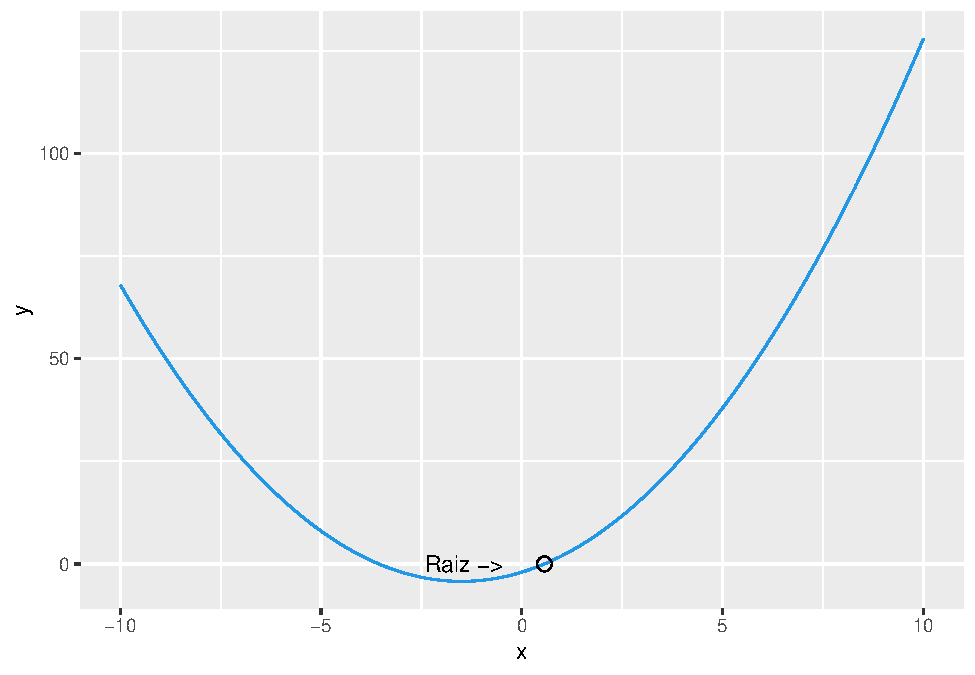
\includegraphics{Newton_raphson_files/figure-latex/unnamed-chunk-4-1.pdf}
\newpage Si deseamos podémos calcular y gráficar ambas raices de la
función.

\begin{Shaded}
\begin{Highlighting}[]
\NormalTok{ráiz_superior <-}\StringTok{ }\KeywordTok{newton}\NormalTok{(fx1,dfx1, limS)}
\NormalTok{ráiz_inferior <-}\StringTok{ }\KeywordTok{newton}\NormalTok{(fx1,dfx1, limI)}
\KeywordTok{ggplot}\NormalTok{(}\DataTypeTok{data=}\NormalTok{ df, }\DataTypeTok{mapping=}\KeywordTok{aes}\NormalTok{(}\DataTypeTok{x=}\NormalTok{ x, }\DataTypeTok{y =}\NormalTok{y))}\OperatorTok{+}
\StringTok{  }\KeywordTok{geom_line}\NormalTok{(}\DataTypeTok{color=}\DecValTok{4}\NormalTok{)}\OperatorTok{+}
\StringTok{  }\KeywordTok{annotate}\NormalTok{(}\DataTypeTok{geom=}\StringTok{"text"}\NormalTok{,}\DataTypeTok{x=}\NormalTok{ráiz_superior}\OperatorTok{+}\DecValTok{2}\NormalTok{, }\DataTypeTok{y=}\DecValTok{0}\NormalTok{, }\DataTypeTok{label=}\StringTok{" <- Ráiz superior "}\NormalTok{)}\OperatorTok{+}
\StringTok{  }\KeywordTok{annotate}\NormalTok{(}\DataTypeTok{geom=}\StringTok{"point"}\NormalTok{, }\DataTypeTok{x=}\NormalTok{ráiz_superior,}\DataTypeTok{y =}\DecValTok{0}\NormalTok{, }\DataTypeTok{size =}\DecValTok{3}\NormalTok{, }\DataTypeTok{shape=}\DecValTok{1}\NormalTok{, }\DataTypeTok{fill=}\StringTok{"transparent"}\NormalTok{)}\OperatorTok{+}
\StringTok{  }\KeywordTok{annotate}\NormalTok{(}\DataTypeTok{geom=}\StringTok{"text"}\NormalTok{,}\DataTypeTok{x=}\NormalTok{ráiz_inferior}\DecValTok{-2}\NormalTok{, }\DataTypeTok{y=}\DecValTok{0}\NormalTok{, }\DataTypeTok{label=}\StringTok{" Ráiz inferior -> "}\NormalTok{)}\OperatorTok{+}
\StringTok{  }\KeywordTok{annotate}\NormalTok{(}\DataTypeTok{geom=}\StringTok{"point"}\NormalTok{, }\DataTypeTok{x=}\NormalTok{ráiz_inferior,}\DataTypeTok{y =}\DecValTok{0}\NormalTok{, }\DataTypeTok{size =}\DecValTok{3}\NormalTok{, }\DataTypeTok{shape=}\DecValTok{1}\NormalTok{, }\DataTypeTok{fill=}\StringTok{"transparent"}\NormalTok{)}
\end{Highlighting}
\end{Shaded}

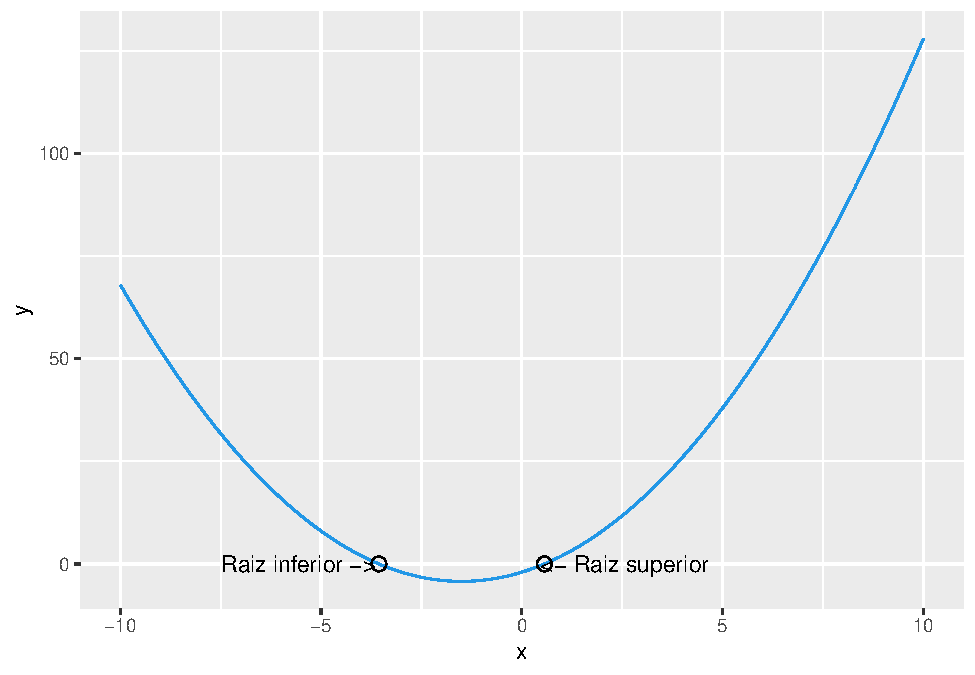
\includegraphics{Newton_raphson_files/figure-latex/unnamed-chunk-5-1.pdf}

\newpage
\singlespacing 
\end{document}